\begin{enumerate}[label=\thesection.\arabic*.,ref=\thesection.\theenumi]
\numberwithin{equation}{enumi}
\item
Sketch direct and inverse polar plots for a unity feedback system with open loop transfer function
\begin{align}
G(s) = \frac{1}{s(1+s)^2}
\end{align}
\\
\solution  
For Unity feedback system, given the open loop transfer function
\begin{align}
G(s) = \frac{1}{s(1+s)^2}
\end{align}
Now, Polar plot is defined as:
The plot of points(represented as $r.e^{j\phi}$) obtained by varying w from 0 to $\infty$  where $r=|H(jw)||G(jw)|$ and $\phi=\angle H(jw)G(jw)$.
\linebreak
Inverse Polar plot is similar, in this $r = \frac{1}{|H(jw)||G(jw)|}$ and $\phi = -\angle H(jw)G(jw)$   
The system we're analysing is unity feedback which means $H(jw) = 1$
Therefore ;
\begin{align}
|H(jw)||G(jw)| = |1|.\frac{1}{|jw||(1+jw)^2|}  
\end{align}
\begin{align}
|H(jw)||G(jw)| = \frac{1}{w(1+w^2)}
\label{eq:mod_G}
\end{align}
and to calculate Phase of G(jw)
\begin{align}
H(jw)G(jw) = 1.e^{0}.1.e^{0}.\frac{1}{w.e^{\pi/2}} . \cbrak{\frac{1}{\sqrt{1^2 + w^2} . e^{tan^{-1}(w)}}}^2  
\end{align}
\begin{align}
H(jw)G(jw) = 1.e^{0}.1.e^{0} w^{-1}.e^{-\pi/2}. (1^2 + w^2)^{-1} . e^{-2tan^{-1}(w)}  
\end{align}
Therefore
\begin{align}
\angle H(jw)G(jw) = \frac{-\pi}{2} - 2tan^{-1}(w)  
\label{eq:phase_G}
\end{align}

The following code plots the polar and inverse polar plots 
%Fig. \ref{fig:sec_order}
\begin{lstlisting}
codes/ee18btech11002/polarplot.py
\end{lstlisting}
\begin{figure}
\centering
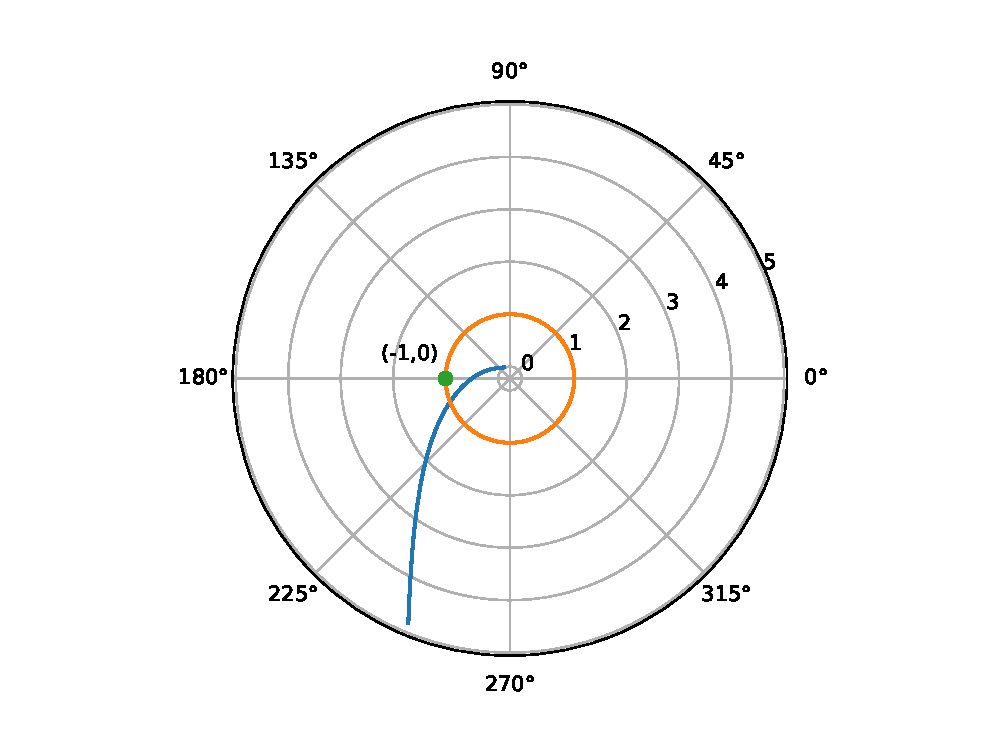
\includegraphics[width=\columnwidth]{./figs/ee18btech11002(a).eps}
\caption{}
\label{fig:polar_plot}
\end{figure}
\begin{figure}
\centering
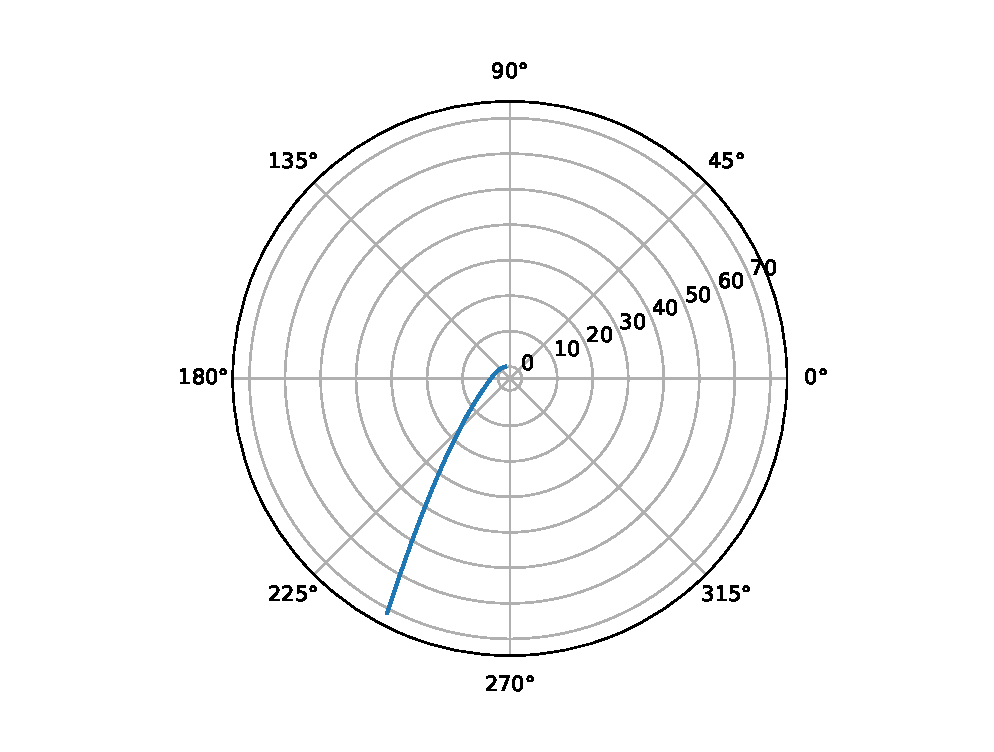
\includegraphics[width=\columnwidth]{./figs/ee18btech11002(b).eps}
\caption{}
\label{fig:inverse_polar_plot}
\end{figure}
 

\item Find the frequency at which $|G(jw)| = 1$ and corresponding phase angle $\angle G(jw)$
\\
\solution 
For $|G(jw)| = 1$
\begin{align}
\frac{1}{w(1+w^2)} = 1
\end{align}
\begin{align}
w + w^3 - 1 = 0
\end{align}
and for the corresponding phase
\begin{align}
\angle G(jw) = \frac{-\pi}{2} - 2tan^{-1}(w)
\end{align}
The following code calculates the value of w and $\angle G(jw)$
%
\begin{lstlisting}
codes/ee18btech11002/solution.py
\end{lstlisting}
%\lstinputlisting{./}
 
%the attached code gives us the solution for the equation
and we get w = 0.682 and $\angle G(jw)=-\frac{52}{59}\pi$


\end{enumerate}
